\newcommand{\walletcollector}{\texttt{wallet\_collector}}
\newcommand{\userinforetriever}{\texttt{user\_info\_retriever}}
\newcommand{\addresschecker}{\texttt{address\_checker}}
\newcommand{\graph}{\texttt{graph}}

\section{Nduja} \label{nduja}

\begin{figure*}
    \centering
    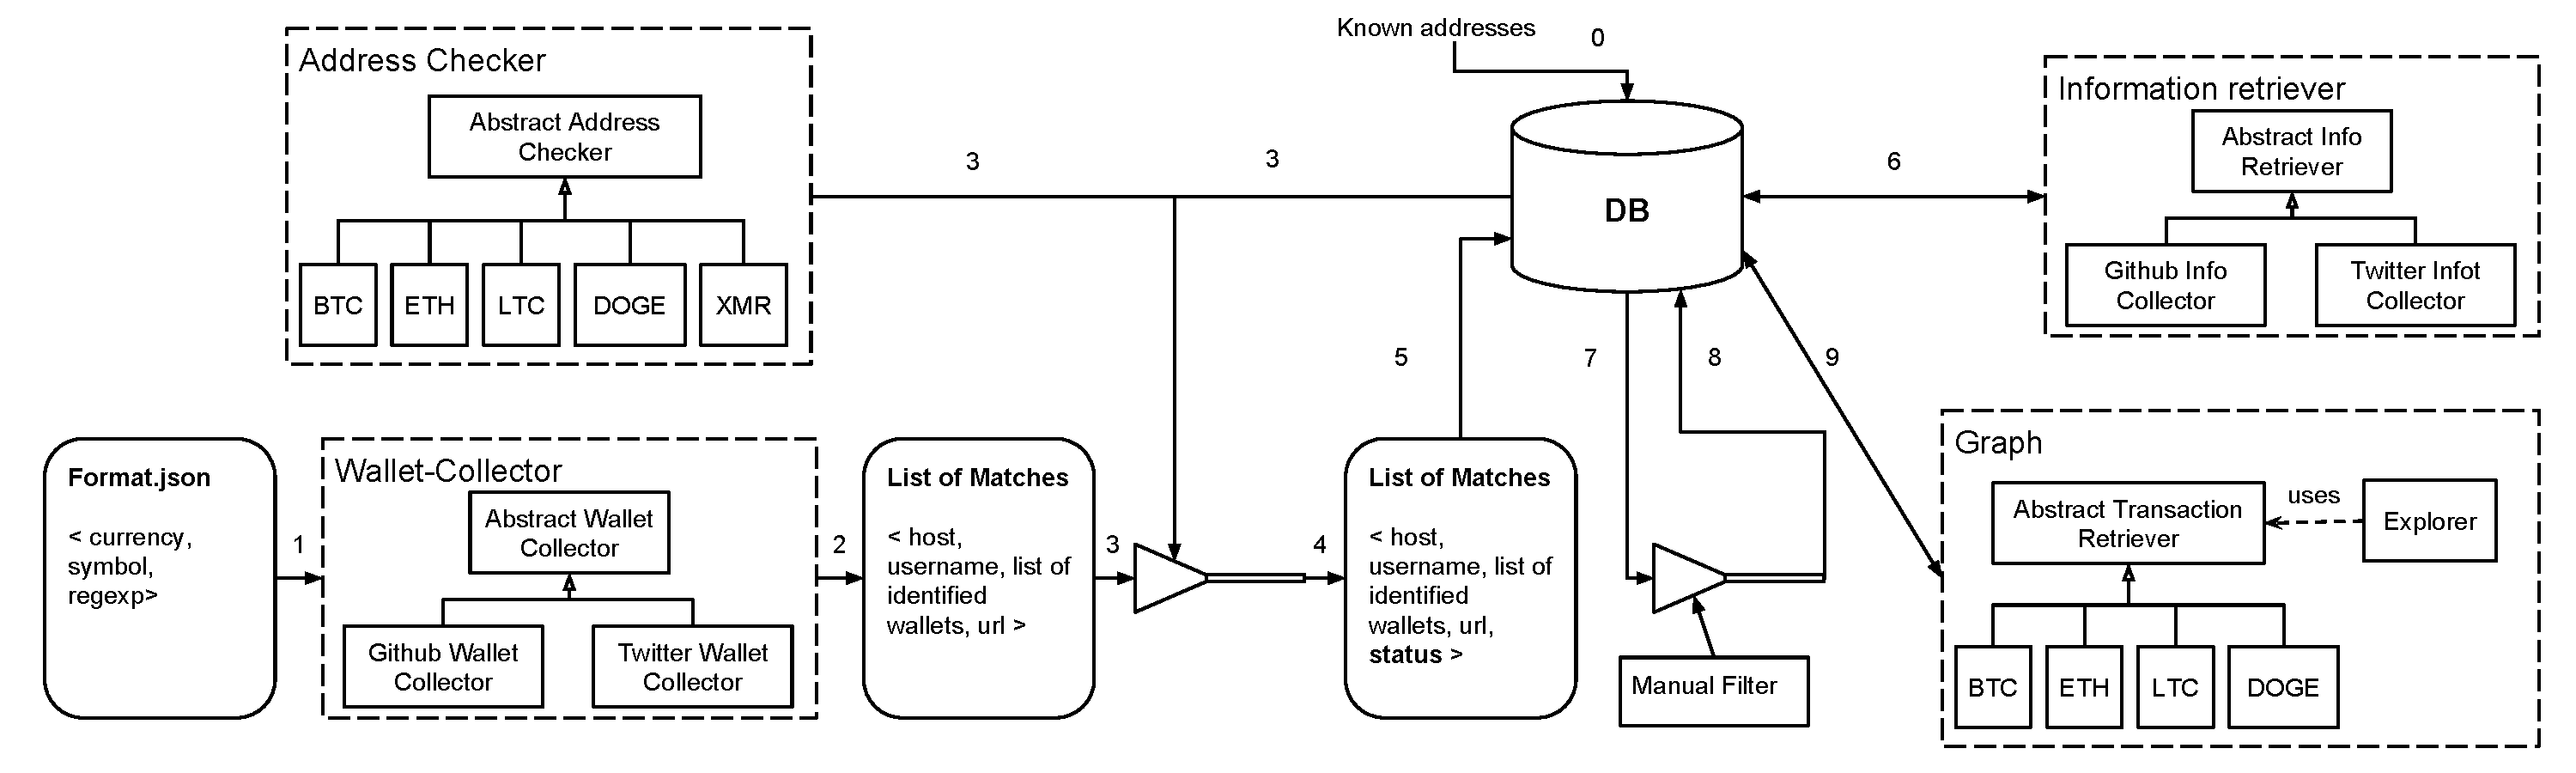
\includegraphics[width=\textwidth]{architecture.pdf}
    \caption{Nduja high level architecture}
    \label{fig:architecture}
\end{figure*}

\subsection{Algorithm}
\texttt{Nduja} algorithm follows a sequence of 3 steps:
\subsubsection*{Data retrieving} Firstly, all possible wallets are collected
from multiple sources and stored in a database along with the
information of where they were retrieved (i.e. reference to the account of the
website in which they are published). In particular in this paper the search is
performed using Github, Twitter and Searchcode API.

\subsubsection*{Account data retrieving} The second step involves the
retrieving of all possible data related to accounts found with the previous
step. This is done by using related APIs (e.g. Twitter API, Github Search API,
Bitbucket API, etc.) to fetch the public information of the accounts and also
by searching for emails and websites in the same resources where we found in
the first place the addresses.

\subsubsection*{Clustering addresses} The last step consists in grouping
wallets that could be associated with the same person: all addresses that are
involved as input of the same transaction can be connected to a single
entity, so we create a ``cluster'' of addresses. In our work to do so we
took advantage of
Blockchain.info API\footnote{\url{https://blockchain.info/api}} and
Chain.so API\footnote{\url{https://chain.so/api}}. These APIs allow
developers to query Bitcoin's, Ethereum's, Litecoin's and Dogecoin's
blockchains without having a local copy of them, that can count
hundreds of gigabytes~\cite{bib:bitinfochart}.

\subsection{Architecture} \label{architecture}
The architecture of Nduja is technology agnostic~\cite{bib:art-of-scalability}
and we chose to implement our prototype with Python\footnote{
	In particular we implemented and tested our system only with versions
	3.5 and 3.6 under Linux environment.} because of its flexibility and
enormous ecosystem.
\autoref{fig:architecture} depicts the architecture of Nduja and its algorithm.
% The dashed boxes represent the main modules of Nduja, the rounded boxes the
% outputs and the numbered arrows the steps of the algorithm.
Before starting the research (0) we filled the database with the addresses of
well-known services, also known as
\emph{tagged addresses}\footnote{\url{https://blockchain.info/tags}}.
The reason to perform this preparatory action 
is twofold: it permits to decrease dramatically the number of
clustered addresses and further tagged addresses are not so
interesting for our purposes because they already voluntarily disclose their
identity.
Then (1) the file \texttt{format.json} is passed to the \verb|wallet_collector|
module. This file contains all the information to build the queries: for each
currency it contains the name (e.g. Bitcoin), the symbol (e.g. BTC) and a
regular expression that is used to collect the wallets inside the texts.
The \verb|wallet_collector| module (2) builds the queries, performs the
researches and find a list of potential matches. To make Nduja extensible it
provides a different class for each different source used, following the same
interface. Indeed it is very easy to add a new source, thanks to the Template
Method Design Pattern.
The list of potential matches is filtered (3) to remove known addresses (taken
from the database) and false matches, that is, addresses that matches the given
regular expressions but are not valid addresses. To perform this latter check
we implemented the module \verb|address_checkers|.
Besides performing validity checks it adds to the list the status, i.e. a
code that is 1 if the wallet performed at least one transaction otherwise 0.
Obviously, after this check the accounts without associated wallets were simply
removed from the list.
Subsequently (5) this list is inserted in the database.
To completely de-anonymize a person we need to gather personal information
about her. Therefore (6) we used the module \verb|user_info_retriever| that
reads the username and the source from the database and searches for its
personal information, collecting personal websites, email and name.
Before proceeding with the clustering we spent a good deal of time (7 and 8)
cleaning the database manually: we focused in searching accounts that were
correlated to a suspiciously high number of wallet correlated or files that
contained a really large set of addresses. By doing this we kept only about 45\%
of the original addresses.
Lastly, (9) we proceed with the clustering procedure exploiting the \verb|graph|
module, that is responsible of analyzing the transactions of the wallets 
inside the database and to find potential overlapping between people in the
database.

\begin{figure*}[h!]
\centering
\begin{subfigure}[t]{0.3\textwidth}
\centering
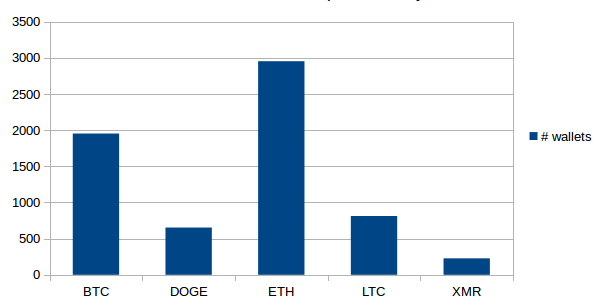
\includegraphics[width=.9\textwidth, height=3.5cm]{number_account_currency}
\caption{Number of wallets retrieved for each currency}
\label{fig:numberaccountcurrency}
\end{subfigure}
~
\begin{subfigure}[t]{0.3\textwidth}
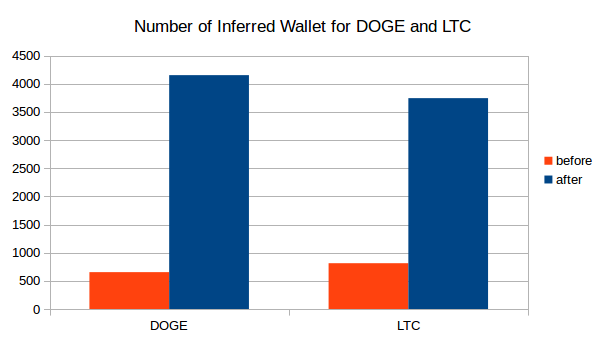
\includegraphics[width=\textwidth, height=3.5cm]{number_inferred_DOGE_LTC}
\caption{Comparison between the number of wallets before and after clustering
for DOGE and LTC}
\label{fig:dogeltcclustered}
\end{subfigure}
~
\begin{subfigure}[t]{0.3\textwidth}
\centering
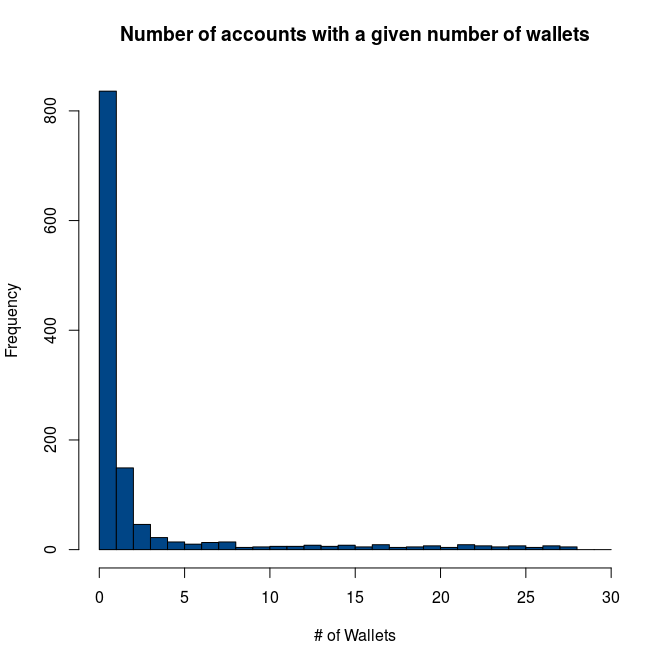
\includegraphics[width=.9\textwidth, height=3.5cm]{numwall}
\caption{Distribution of the number of wallets per account}
\label{fig:numwall}
\end{subfigure}
\caption{Results of our study}
\end{figure*}

\subsection{Queries}
\label{sec:queries}
To maximize the number of possible results in repositories the module
\walletcollector{} searches for files that contain words such as
\textbf{donation} or \textbf{contribution} and in which there is a set of
characters that matches the provided regular expressions defined for the
different address formats. This has been implemented using two different APIs:
Github Search API\footnote{\url{https://developer.github.com/v3/search/}} and
Searchcode API\footnote{\url{https://searchcode.com/api/}}.
In addition to the keywords searched in Github, in Twitter we searched also for
\textit{hashtags} such as \textbf{\#GiveAway} and
hashtags correlated to specific cryptocurrency (e.g. \#BTCGiveAway). This has
been done using Twitter
API\footnote{\url{https://developer.twitter.com/en/docs/api-reference-index}}.
However, it has a strong limitation: we are only able to retrieve tweets that
were published at most a week before the search. This limitation is imposed
because we have not paid for a premium account. In fact our research must be
thought as a proof of concept.
Although this limitation even with a free account one can collect a huge amount
of data by performing those queries weekly:
the information before the first search is lost without a premium account, but,
following this idea it is possible to collect incrementally all the future
addresses.

\subsection{Database}
All data retrieved is stored into a
SQLite\footnote{\url{https://www.sqlite.org/}} database. The information stored
for a user are the name, websites and emails, along with the response of the
request
with which the information is carried out. Addresses are recorded alongside the
URL in which they were found. Moreover each address is flagged with a
field that could be: \texttt{0} if the address is not used yet, \texttt{1}
whether the address is used at least for one transaction or \texttt{-1} when it
is tagged address.